\documentclass[12pt,a4paper]{article}
\usepackage[utf8]{vietnam}
\usepackage{amsmath,amssymb}
\usepackage{tabularx}
\usepackage{tikz}
\usetikzlibrary{calc,angles,quotes,arrows.meta,patterns}
\usepackage{xcolor}
\usepackage{enumitem}
\usepackage{fancyhdr}
\usepackage[top=1.2cm, bottom=1.2cm, left=1.5cm, right=1.5cm]{geometry}
\usepackage[dethi]{ex_test}
\SAOPTN{widthSA=2.6,heightSA=0.62}

\setlength{\headheight}{15pt}
\setlength{\parskip}{0pt}

\pagestyle{fancy}
\fancyhf{}
\rhead{\textit{Môn Toán 6 -- Đề số 11}}
\lhead{\textit{Bộ đề ôn tập Giữa học kì I}}
\cfoot{\thepage}

\begin{document}

% --- KHUNG TIÊU ĐỀ ĐỀ THI ---
\noindent
\begin{tabularx}{\linewidth}{X r}
\textbf{TRƯỜNG THCS: \dotfill} & \textbf{ĐỀ KIỂM TRA ĐỊNH KỲ GIỮA HỌC KỲ I} \\
\textbf{Họ và tên: \dotfill} & \textbf{NĂM HỌC 2026 -- 2027} \\
\textbf{Lớp: \dotfill \quad SBD: \dotfill} & \textbf{Môn: TOÁN 6} \\
\hline
\end{tabularx}
\vspace{2mm}

\begin{center}
  \textbf{\large ĐỀ ÔN TẬP GIỮA HỌC KỲ I -- ĐỀ SỐ 11}\\
  \textit{Thời gian làm bài: 90 phút (Không kể thời gian phát đề)}
\end{center}
\vspace{1mm}

% --- PHẦN I ---
\noindent\textbf{\large PHẦN I. CÂU TRẮC NGHIỆM NHIỀU PHƯƠNG ÁN LỰA CHỌN (3,0 điểm)}

\textit{Thí sinh trả lời từ câu 1 đến câu 12. Mỗi câu hỏi thí sinh chỉ chọn một phương án duy nhất.}

\vspace{1mm}
\begin{ex}
Trong các số sau, số nào là bội của 5?
\choice
{$7$}
{\True $105$}
{$17$}
{$27$}
\end{ex}

\begin{ex}
Tìm $x$, biết $x + 20 = 42$:
\choice
{\True $22$}
{$62$}
{$2$}
{$18$}
\end{ex}

\begin{ex}
Khẳng định nào sau đây là đúng?
\choice
{$4 \in Ư(7)$}
{$5 \in Ư(7)$}
{$6 \in Ư(7)$}
{\True $7 \in Ư(7)$}
\end{ex}

\begin{ex}
Cho $x \in \{5; 16; 25; 135\}$ sao cho tổng $20 + 35 + x$ không chia hết cho 5. Khi đó $x$ có thể là:
\choice
{$5$}
{\True $16$}
{$25$}
{$135$}
\end{ex}

\begin{ex}
Trong các số sau, số nào chia hết cho cả 2 và 5?
\choice
{\True $2020$}
{$25$}
{$52$}
{$5$}
\end{ex}

\begin{ex}
Tổng $3510 + 4353$ chia hết cho:
\choice
{$2$}
{\True $3$}
{$5$}
{$9$}
\end{ex}

\begin{ex}
Hình nào dưới đây là tam giác đều?
\begin{center}
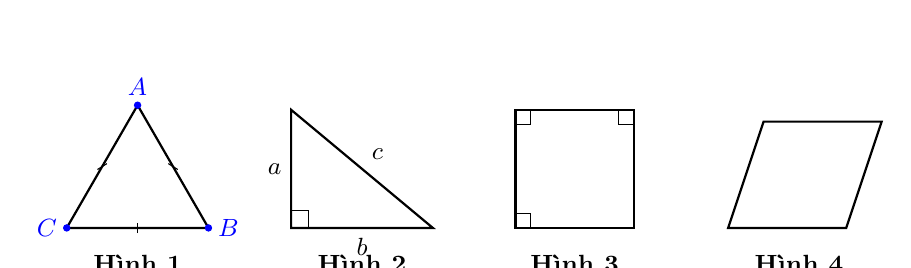
\begin{tikzpicture}[scale=0.75, font=\small]
  \begin{scope}[shift={(0,0)}]
    \coordinate (C) at (0,0); \coordinate (B) at (2.4,0); \coordinate (A) at (1.2, 2.078);
    \draw[thick] (A) -- (B) -- (C) -- cycle;
    \filldraw[blue] (A) circle (1.5pt) node[above] {$A$};
    \filldraw[blue] (B) circle (1.5pt) node[right] {$B$};
    \filldraw[blue] (C) circle (1.5pt) node[left] {$C$};
    \draw ($(A)!0.5!(B) + (-0.08,0.05)$) -- ($(A)!0.5!(B) + (0.08,-0.05)$);
    \draw ($(A)!0.5!(C) + (-0.08,-0.05)$) -- ($(A)!0.5!(C) + (0.08,0.05)$);
    \draw ($(B)!0.5!(C) + (0,-0.09)$) -- ($(B)!0.5!(C) + (0,0.09)$);
    \node at (1.2, -0.6) {\textbf{Hình 1}};
  \end{scope}
  \begin{scope}[shift={(3.8,0)}]
    \coordinate (V) at (0,0); \coordinate (X) at (2.4,0); \coordinate (Y) at (0,2);
    \draw[thick] (V) -- (X) -- (Y) -- cycle; \draw (0,0.3) -- (0.3,0.3) -- (0.3,0);
    \node[left] at (0,1) {$a$}; \node[below] at (1.2,0) {$b$}; \node[above right] at (1.2,1) {$c$};
    \node at (1.2, -0.6) {\textbf{Hình 2}};
  \end{scope}
  \begin{scope}[shift={(7.6,0)}]
    \coordinate (D) at (0,0); \coordinate (C3) at (2,0); \coordinate (B3) at (2,2); \coordinate (A3) at (0,2);
    \draw[thick] (A3) -- (B3) -- (C3) -- (D) -- cycle;
    \draw (0,1.75) -- (0.25,1.75) -- (0.25,2); \draw (2,1.75) -- (1.75,1.75) -- (1.75,2); \draw (0,0.25) -- (0.25,0.25) -- (0.25,0);
    \node at (1, -0.6) {\textbf{Hình 3}};
  \end{scope}
  \begin{scope}[shift={(11.2,0)}]
    \coordinate (D4) at (0,0); \coordinate (C4) at (2,0); \coordinate (B4) at (2.6,1.8); \coordinate (A4) at (0.6,1.8);
    \draw[thick] (A4) -- (B4) -- (C4) -- (D4) -- cycle;
    \node at (1.2, -0.6) {\textbf{Hình 4}};
  \end{scope}
\end{tikzpicture}
\end{center}
\choice
{\True Hình 1}
{Hình 2}
{Hình 3}
{Hình 4}
\end{ex}

\begin{ex}
Kết quả của $7^{56} : 7^{51}$ viết dưới dạng một lũy thừa là:
\choice
{\True $7^5$}
{$7^6$}
{$7^{107}$}
{$7^4$}
\end{ex}

\begin{ex}
Trong các hình dưới đây, hình nào là tam giác đều?
\begin{center}
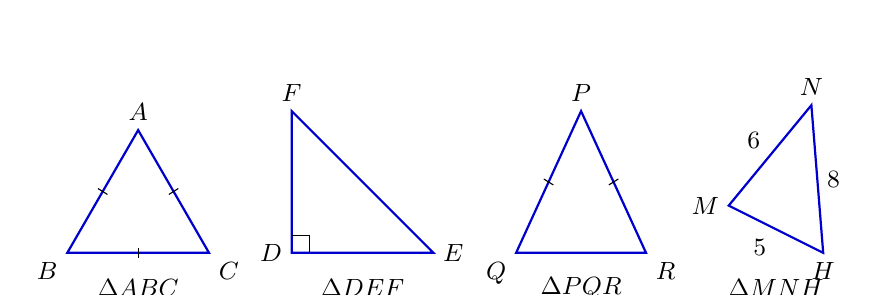
\begin{tikzpicture}[scale=0.75, font=\small]
  \begin{scope}[shift={(0,0)}]
    \coordinate (B) at (0,0); \coordinate (C) at (2.4,0); \coordinate (A) at (1.2, 2.078);
    \draw[thick, blue!80!black] (A) -- (B) -- (C) -- cycle;
    \node[above] at (A) {$A$}; \node[below left] at (B) {$B$}; \node[below right] at (C) {$C$};
    \draw ($(A)!0.5!(B) + (-0.08,0.05)$) -- ($(A)!0.5!(B) + (0.08,-0.05)$);
    \draw ($(A)!0.5!(C) + (-0.08,-0.05)$) -- ($(A)!0.5!(C) + (0.08,0.05)$);
    \draw ($(B)!0.5!(C) + (0,-0.09)$) -- ($(B)!0.5!(C) + (0,0.09)$);
    \node at (1.2, -0.6) {$\Delta ABC$};
  \end{scope}
  \begin{scope}[shift={(3.8,0)}]
    \coordinate (D) at (0,0); \coordinate (E) at (2.4,0); \coordinate (F) at (0,2.4);
    \draw[thick, blue!80!black] (D) -- (E) -- (F) -- cycle; \draw (0,0.3) -- (0.3,0.3) -- (0.3,0);
    \node[left] at (D) {$D$}; \node[right] at (E) {$E$}; \node[above] at (F) {$F$};
    \node at (1.2, -0.6) {$\Delta DEF$};
  \end{scope}
  \begin{scope}[shift={(7.6,0)}]
    \coordinate (Q) at (0,0); \coordinate (R) at (2.2,0); \coordinate (P) at (1.1,2.4);
    \draw[thick, blue!80!black] (P) -- (Q) -- (R) -- cycle;
    \node[above] at (P) {$P$}; \node[below left] at (Q) {$Q$}; \node[below right] at (R) {$R$};
    \draw ($(P)!0.5!(Q) + (-0.08,0.05)$) -- ($(P)!0.5!(Q) + (0.08,-0.05)$);
    \draw ($(P)!0.5!(R) + (-0.08,-0.05)$) -- ($(P)!0.5!(R) + (0.08,0.05)$);
    \node at (1.1, -0.6) {$\Delta PQR$};
  \end{scope}
  \begin{scope}[shift={(11.2,0)}]
    \coordinate (M) at (0,0.8); \coordinate (H) at (1.6,0); \coordinate (N) at (1.4,2.5);
    \draw[thick, blue!80!black] (M) -- (H) -- (N) -- cycle;
    \node[left] at (M) {$M$}; \node[below] at (H) {$H$}; \node[above] at (N) {$N$};
    \node[below left] at (0.8,0.4) {$5$}; \node[above left] at (0.7,1.6) {$6$}; \node[right] at (1.5,1.25) {$8$};
    \node at (0.8, -0.6) {$\Delta MNH$};
  \end{scope}
\end{tikzpicture}
\end{center}
\choice
{\True Tam giác $ABC$}
{Tam giác $DEF$}
{Tam giác $PQR$}
{Tam giác $MNH$}
\end{ex}

\begin{ex}
Cho hình bình hành $AKHE$ có $AK = 6\text{ cm}, KH = 5\text{ cm}$. Hãy chọn phát biểu đúng trong các phát biểu sau:
\choice
{$EH = 5\text{ cm}, AE = 6\text{ cm}$}
{\True $EH = 6\text{ cm}, AE = 5\text{ cm}$}
{$AH = 6\text{ cm}, AE = 5\text{ cm}$}
{$KH = 6\text{ cm}, AH = 5\text{ cm}$}
\end{ex}

\begin{ex}
Tập hợp $L = \{x \in \mathbb{N}^* \mid x \text{ là số lẻ và } x \le 9\}$ được viết dưới dạng liệt kê các phần tử là:
\choice
{$\{1; 3; 5; 7\}$}
{\True $\{1; 3; 5; 7; 9\}$}
{$\{1; 2; 3; 4; 5; 6; 7; 8\}$}
{$\{1; 2; 3; 4; 5; 6; 7; 8; 9\}$}
\end{ex}

\begin{ex}
Chu vi hình thoi $MNPQ$ có cạnh $MN = 5\text{ cm}$ là:
\choice
{\True $20\text{ cm}$}
{$15\text{ cm}$}
{$25\text{ cm}$}
{$10\text{ cm}$}
\end{ex}


\vspace{1mm}
\noindent\textbf{BẢNG TRẢ LỜI TRẮC NGHIỆM PHẦN I:}
\begin{center}
\begin{tabular}{|c|c|c|c|c|c|c|c|c|c|c|c|c|}
\hline
\textbf{Câu} & \textbf{1} & \textbf{2} & \textbf{3} & \textbf{4} & \textbf{5} & \textbf{6} & \textbf{7} & \textbf{8} & \textbf{9} & \textbf{10} & \textbf{11} & \textbf{12} \\
\hline
\textbf{Chọn} & \rule{0pt}{0.65cm} & & & & & & & & & & & \\
\hline
\end{tabular}
\end{center}
\vspace{2mm}

\setcounter{ex}{0}
\noindent\textbf{\large PHẦN II. CÂU TRẮC NGHIỆM ĐÚNG SAI (2,0 điểm)}

\textit{Thí sinh trả lời câu 1 và câu 2. Trong mỗi ý a), b), c), d) ở mỗi câu, thí sinh chọn đúng hoặc sai.}

\vspace{1mm}
\begin{ex}
Xét tính đúng/sai của các mệnh đề sau:
\choiceTF
{Mọi số có chữ số tận cùng là 3; 6; 9 thì chia hết cho 3}
{Để số $\overline{212*}$ chia hết cho 2 thì $* \in \{4; 6; 8\}$}
{\True Số chia hết cho 9 thì số đó chia hết cho 3}
{\True Các số có chữ số tận cùng là 0 hoặc 5 thì chia hết cho 5}
\end{ex}

\begin{ex}
Cho các số $a = 12, b = 18$ và $c = 30$. Xét tính đúng/sai của các mệnh đề sau:
\choiceTF
{\True Số $a$ là bội của 4}
{\True Số 6 là ước chung của cả ba số $a, b, c$}
{Ước chung lớn nhất của $a$ và $b$ là 12}
{\True Bội chung nhỏ nhất của $a$ và $b$ là 36}
\end{ex}


\noindent\textbf{BẢNG TRẢ LỜI PHẦN II:}
\begin{center}
\begin{tabular}{|c|c|c|c|c||c|c|c|c|c|}
\hline
\textbf{Câu 1} & \textbf{a)} & \textbf{b)} & \textbf{c)} & \textbf{d)} & \textbf{Câu 2} & \textbf{a)} & \textbf{b)} & \textbf{c)} & \textbf{d)} \\
\hline
\textbf{Đ/S} & \rule{0pt}{0.6cm} & & & & \textbf{Đ/S} & & & & \\
\hline
\end{tabular}
\end{center}
\vspace{2mm}

\setcounter{ex}{0}
\noindent\textbf{\large PHẦN III. CÂU HỎI TRẢ LỜI NGẮN (2,0 điểm)}

\textit{Thí sinh trả lời câu 1 và câu 2. Điền kết quả số vào ô trống tương ứng.}

\vspace{1mm}
\begin{ex}
Một hình lục giác đều có độ dài một cạnh bằng $5\text{ cm}$. Tính chu vi của hình lục giác đều đó (theo đơn vị $\text{cm}$). \shortans{30}
\end{ex}

\begin{ex}
Một khu vườn hình chữ nhật có chiều dài $15\text{ m}$ và chiều rộng $10\text{ m}$. Người ta làm hàng rào xung quanh khu vườn và để lại một cửa ra vào rộng $2\text{ m}$. Tính độ dài của hàng rào đó (theo đơn vị $\text{m}$). \shortans{48}
\end{ex}


\setcounter{ex}{0}
\noindent\textbf{\large PHẦN IV. TỰ LUẬN (3,0 điểm)}

\textit{Thí sinh trình bày chi tiết lời giải vào giấy làm bài.}

\vspace{1mm}
\begin{ex} (1,0 điểm)
Tìm số tự nhiên $x$, biết:
\begin{enumerate}[label=\textbf{\alph*)}, leftmargin=0.8cm, itemsep=2pt]
\item (0,5 điểm) $x + 37 = 50$
\item (0,5 điểm) $(x + 2) : 5 = 6$
\end{enumerate}
\end{ex}
\vspace{1.5mm}

\begin{ex} (1,0 điểm)
Tập hợp và bài toán thực tế tiết kiệm:
\begin{enumerate}[label=\textbf{\alph*)}, leftmargin=0.8cm, itemsep=2pt]
\item (0,5 điểm) Viết tập hợp $A$ các số tự nhiên nhỏ hơn 8. Liệt kê các số nguyên tố trong tập hợp $A$?
\item (0,5 điểm) Mỗi tháng An tiết kiệm $35\,000$ đồng để mua một đôi giày thể thao. Sau 1 năm, An đã mua được đôi giày và còn lại $23\,000$ đồng. Hỏi đôi giày An mua giá bao nhiêu đồng?
\end{enumerate}
\end{ex}
\vspace{1.5mm}

\begin{ex} (0,5 điểm)
Một khu vườn hình chữ nhật có chiều dài $20\text{ m}$, chiều rộng ít hơn chiều dài $5\text{ m}$. Người ta dự định rào xung quanh khu đất bằng 4 đường dây kẽm gai để trồng rau.
\begin{enumerate}[label=\textbf{\alph*)}, leftmargin=0.8cm, itemsep=2pt]
\item (0,25 điểm) Hỏi cần tất cả bao nhiêu mét dây kẽm gai để rào khu đất trên?
\item (0,25 điểm) Người nông dân thu hoạch được bao nhiêu kg rau trên khu vườn này, biết rằng cứ $1\text{ m}^2$ thu hoạch được $2\text{ kg}$ rau, diện tích lối đi và hệ thống thoát nước là $50\text{ m}^2$?
\end{enumerate}
\end{ex}
\vspace{1.5mm}

\begin{ex} (0,5 điểm)
Không thực hiện tính tổng, chứng minh rằng $A = 1 + 4 + 4^2 + 4^3 + \dots + 4^{2021}$ chia hết cho 21.
\end{ex}
\vspace{1.5mm}


\begin{center}
\rule{4cm}{0.4pt}\\
\textit{--- HẾT ---}
\end{center}
\end{document}
